\documentclass[letterpaper]{article}

\usepackage{aaai}
\usepackage{prasem}

\begin{document}

\title{Rough Set Semantics for Identity on the Web}
\author{Wouter Beek \and Stefan Schlobach \and Frank van Harmelen\\
Vrije Universiteit Amsterdam\\
De Boelelaan 1081a\\
1081HV Amsterdam\\
The Netherlands}
\maketitle
\begin{abstract}
\begin{quote}
Identity relations are at the foundation of the Linked Open Data initiative
  and on the Semantic Web in general.
They allow the interlinking of alternative descriptions of the same thing.
However, many practical uses of \verb|owl:sameAs| are known to violate its
  formal semantics.
We propose a method that assigns meaning to (the subrelations of)
  an identity relation using the predicates of the dataset schema.
Applications of this approach include automated suggestions for
  asserting/retracting identity pairs and quality assessment.
We also describe an experimental design for this approach.
\end{quote}
\end{abstract}

% Section 1: Introduction
\section{Introduction}
\label{sec:introduction}

Identity relations are at the foundation of the Linked Open Data initiative
  and of the Semantic Web in general \cite{bizer_cyganiak_heath_2007}.
They allow the interlinking of alternative descriptions of the same thing.
However, the traditional notion of identity
  (expressed by \verb|owl:sameAs| \cite{motic_paterschneider_grau_2012})
  is often problematic, e.g. when objects are considered the same in some
  contexts but not in others.
The standing practice in such cases is to use weaker relations of relatedness
  (e.g., \verb|skos:related|).
Unfortunately, this limits reasoners in drawing inferences.

According to the traditional semantics of the identity relation,
  identical terms can be replaced for one another in all non-modal contexts
  \emph{salva veritate}.
Practical uses of \verb|owl:sameAs| are known to violate this strict condition
  \cite{halpin_hayes_2010,halpin_hayes_mccusker_mcguinness_thompson_2010}.

Identity is often thought of as having the exact same properies.
This statement is known as the Principle of indiscernibility
(see \ref{def:indiscernibility_of_identicals})
and has been attributed to Leibniz.\cite{TODO}
% Gottfried Wilhelm Leibniz, section 9, Discourse on Metaphysics.

\begin{definition}[Indiscernibility of identicals]
\label{def:indiscernibility_of_identicals}
$a = b \rightarrow (\forall \phi \in \Phi) \phi(a) = \phi(b)$
\end{definition}

Although the principle provides necessary and sufficient conditions
for identity, it does not point us to an automated procedure
for enumerating the extension of the identity relation.
Due to its circular nature the set of properties includes
``being identical to $x$'' (for every resource $x$).

But even though this priciple does not
allow a positive identification of identity pairs,
it does provide an exclusion condition,
namely resources that are known to not share some property
are also known to not be identical.

\subsection{Generic problems of identity}

Identity poses several problems which are not specific to the SW.
Firstly, it does not hold across modal contexts,
e.g. allowing Louis Lane to believe that Superman saved her,
without her knowling that Clark Kent saved here.
Secondly, identity seems to be a relative concept\cite{Geach},
e.g. two medicines may be the same chemical \emph{substance}
while not being the same \emph{medicine}.
Thirdly, identity over time poses problems,
since a ship may be considered the same
even though all components from which it was built
have been changed over the course of time.\cite{}
Lastly, the problem of identity under counterfactual assertions
such as ``If Obama would have been bron outside of the US,
then he would not have been president of the US today.''\cite{Kripke1980}

\subsection{SW-specific problems of identity: Semantics}

Besides the generic problems of identity,
there are problems that are specific to the SW.
The first SW-specific problem follows from its semantics;
the second one follows from its pragmatics.

Firstly, in the context of the SW\footnote{
\begin{definition}[Semantics of \verb|owl:sameAs|]
\label{def:owl_sameAs}
$\langle a_1, a_2 \rangle \in Ext(I(\texttt{owl:sameAs})) \iff a_1 = a_2$
\end{definition}
},
identity assertions are extra strong
because of the Open World Assumption.
Stating that two resources are the same
implies that from now on no new property can be added
to only one of those resources.
When we formulate this in terms of
principle \ref{def:indiscernibility_of_identicals},
we can say that in the SW the set $\Phi$ contains
all the properties that can \emph{possibly} be expressed
in the modeling language.
This is obviously much bigger than the actual vocabulary
of any in use dataset.

Moreover, whether or not two resources share the absence of a \emph{property}
(i.e., a property of the form ``does not have the property $\phi$''),
cannot be concluded based on the absence of a \emph{property assertion}.
Such `negative knowledge' must be provided explicitly
using class restrictions.

\subsection{SW-specific problems of identity: Pragmatics}

Besides the semantic SW-specific problem,
we can identify a pragmatic SW-specific problem of identity.

The SW is not only a formal model,
it is also a social construct which evolves over time
(like the syntactic Web).
When we look at the SW as a social machine\cite{TODO},
% REF http://sociam.org/www2013/
% WWW2013 Workshop
% The Theory and Practice of Social Machines
we observe that modelers have different opinions regarding whether
two resources are identical or not.

Modelers are known not to conform to the strict semantics of identity\footnote{
  At the AAAI Fall Symposium 2013 track on Semantics for Big Data
  the problem of identity was considered to be one of the most
  relevant problems facing the Semantic Web today.
},
and it is unlikely that all who contribute to the SW are able to
quantify over the entire realm of possible properties
(i.e., $\Phi$ in principle \ref{def:principle_of_indiscernibility}).
Practice shows that two modeler sometimes have different opinions,
the one claiming resources to be identical,
whereas another considers them to be only (closely) related.

As a social system, the SW has semantics and pragmatics.
The pragmatics of the SW are encoded in the open-ended collection of
common practices that effectuate the creation and usage of SW content.
An example of such an encoded common practice are the five `stars'
of Linked Open Data (LOD) publishing.\cite{TODO}
These five `stars' are effectively five \emph{maxims} that specify
(part of) the pragmatics of LOD publishing,
just like the Gricean maxims specify
(part of) the pragmatics of natural language discourse.\cite{TODO}
% Grice

The fifth `star' or maxim reads:
``Link your data to other people\'s data to provide context.''
Given that RDF links are often specified using
the \verb|owl:saveAs| predicate\cite{void},
%``RDF links often have the owl:sameAs predicate.'' [VoID]
we conclude that the pragmatics of the SW are orthogonal to its semantics.

The the pragmatics of the SW, observed in contemporary common practices,
states that by asserting identity between resources,
more context is added for those resources
(since this results in more triples being asserted about the same resource).
At the same time we see that the semantics of identity
gets violated once the context in which a resource was created
is extended (by identity assertions) beyond this original context.
(This is true regardless of whether context is defined in terms of
`intended use', `domain', `time', or `modality'.

From the social point of view
we see that the requirements on SW modelers
are unreasonably high when they are required to
assert identity links in accordance with the semantics.
At the same time the pragmatics states that modelers should
make those links.



What we are left with is a very strong identity claim
which allows statements such as:
``Medicines $a$ and $b$ are the same because they have the exact same
  chemical composition'',
thereby disallowing another SW contributor to state that
$a$ and $b$ are produced by different companies.

\subsection{Research goals}
\label{sec:research_goals}

In developing our approach we have the following research goals:
\begin{enumerate}
\item In an identity relation the pairs all look the same.
      We want to characterize subrelations of an identity relation in terms
      of the predicates that occur in the schema of the dataset.
\item Based on an existing identity relation we want to give semantically
      motivated suggestions for extending/limiting the identity relation.
\item We want to assess the quality of an identity relation based on
      the consistency with which it is applied to the data.
\end{enumerate}

\section{Related work}
\label{sec:related_work}

Existing research suggests six different solutions for
  the problem of identity on the SW.

\textbf{[1] Introduce weaker versions of {\small \texttt{owl:sameAs}}}
  \cite{HalpinHayes2010,MccuskerMcguinness2010}.
Candidates for replacement are
  the SKOS concepts
  {\small \texttt{skos:related}} and {\small \texttt{skos:exactMatch}}
  \cite{MilesBechhofer2009}.
The former is not transitive,
  thereby limiting the possibilities for reasoning.
The latter is transitive,
  but can only be used in certain contexts.
It is not defined in what contexts it can be used
  \cite{MilesBechhofer2009}.\footnote{
    For instance, the property {\small \texttt{skos:exactMatch}}
    ``is used to link two concepts, indicating a high degree of confidence
    that the concepts can be used interchangeably across a wide range of
    information retrieval applications.''
  }
\begin{comment}
% SIMILARITY
The problem with using weaker notions such as relatedness,
  is that everything is related to everything in \emph{some} way.}
% Shall we discuss similarity here as well?
% Does similarity differ from relatedness?
\end{comment}

\textbf{[2] Restrict the applicability of identity relations}
  to specific contexts.
In terms of Semantic Web technology, identities are expected to hold
  within a named graph or within a namespace,
  but not necessarily outside of it \cite{HalpinHayes2010}.
\cite{Melo2013} has succesfully used the Unique Names Assumption
  within namespaces in order to identify many (arguably) spurious
  identity statements.

\textbf{[3] Introduce additional vocabulary} that does not weaken but extends
  the existing identity relation.
\cite{HalpinHayes2010} mention an explicit distinction that could be made
  between mentioning a term and using a term,
  thereby distinguishing an object and a Web document describing that object.
Other possible extensions of {\small \texttt{owl:sameAs}} might take
  the Fuzzyness and/or uncertainty of identity statements into account.

\textbf{[4] Use domain-specific identity relations}
  \cite{MccuskerMcguinness2010}.
For instance
    ``$x$ and $y$ have the same medical use''
  replaces
    identity in the domain of medicine,
and
    ``$x$ and $y$ are the same molecule''
  replaces
    identity in the domain of chemistry.
The downside to this solution is that domain-specific links are
  only locally valid, thereby limiting knowledge reuse.

\textbf{[5] Change the modeling practice}, possibly in a (semi-)automated way
  by adapting visualization and modeling toolkits to produce notifications
  upon reading SW data, or by posing additional restrictions on the creation
  and alteration of data. For example, adding an RDF link could require
  reciprocal confirmation from the maintainers of the respective datasets.
  \cite{HalpinHayes2010,DingShinavierFininMcguinness2010}
The problem with introducing checks and ballances on editing operations,
  is that it violates one of the fundamental underpinnings of the SW;
  namely that on the Web of Data anybody is allowed to say
  anything about anything \cite{AntoniouGrothHarmelenHoekstra2012}.

\textbf{[6] Extract network properties of {\small \texttt{owl:sameAs}}
  datasets} \cite{DingShinavierShangguanMcguinness2010}.
Although this work shows that network analysis can provide insights
  into the ways in which identity is used in the SW,
  these endeavors have not yet been related to the semantics of the
  identity relation.
We believe that utilizing network theoretic aspects in order to
  determine the meaning of identity statements
  would be interesting future research.

What the existing approaches have in common is
  that quite some work has to be done
  (adapting or creating standards, instructing modelers, converting existing
  datasets) in order to resolve only some of the problems of identity.
Our approach provides a way of dealing with the heterogeneous real-world
  usage of identity in the SW that is fully automated and requires
  no changes to standards, modeling practices, or existing datasets.


% Section 2: Approach
\section{Approach}
\label{sec:approach}

First we give a short outline of our approach and then
  we provide a more detailed description of the individual steps.

\subsection{Outline of the approach}

We start by assuming that we are given an identity relation $\approx$.
We will then reinterpret this relation as an indiscernibility relation
  relative to different sets of predicates.
Pairs that have the same indiscernibility predicates
  are simi-discernible, i.e.: they discern resources
  based on the same criteria.
Simi-discernibility is an equivalence relation
  which partitions all pairs and thus also the identity relation $\approx$.
The members of the indiscernibility partition
  have a certain overlap with the original identity relation.
The overlap between an indiscernibility subset and the identity relation
  is called an \emph{identity subrelation}.
Each identity subrelation is characterized in terms of predicates
  from the domain vocabulary.
Different forms of identity can therefore be distinguished
  and meaningfully described.
Based on whether there is a complete or a partial overlap
  between the simi-discernible partition members and
  the identity subrelations,
  these partition members belong either to the lower ($\lowerapprox$)
  or to the higher approximation ($\higherapprox$) of $\approx$.
Besides setting a lower and a higher bound to the identity relation,
  we can also calculate the quality of the identity relation
  and the precision of each identity subrelation.

\subsection{Preliminaries}
\label{sec:preliminaries}

%TODO 'reosurce'->'object'
%TODO explain that 'objects' are not 'object terms'
%     and are not even (always) denoted by object terms.

$G$ denotes an RDF graph. It consists of a set of ground binary
predicates $p(s,o)$, called ``triples'' in Semantic Web jargon, and often
written as $\triple{s}{p}{o}$. These triples form a graph with all
subjects $s$ and objects $o$ as nodes, and 
each assertion $p(s,o)$ corresponding to a directed edge labelled $p$
between $s$ and $o$. 

We assume that graphs are always closed under
  RDFS and OWL-DL entailment
  (see section \ref{sec:implementation} for details).

We identify subsets of RDF terms based on
  their positional occurrence in triples in $G$:
  $S_G$, $P_G$, and $O_G$ denote the subject, predicate and object terms
  in $G$ respectively.

The interpretation $I$ maps RDF terms onto resources,
  and triples onto truth values.
The extension function $Ext$ maps resources onto pairs of resources.
$I(\triple{s}{p}{o})$ is true iff
  $\pair{I(s)}{I(o)} \in Ext(I(p))$ \cite{Hayes2004}.

A note on terminology: Our use of the word `property' does not coincide
  with the notion of an RDF property, but is closer to the notion
  of a FOL property. Our use of the word `relation' will be close to
  both the notion of a FOL relation and the notion of an RDF property.
  We briefly explain the distinctions.

An RDF property is a resource (i.e., a member of the domain)
  that is the interpretation of
  an RDF term that occurs in the predicate position of a triple.\footnote{
    Notice that we do not use the posibility modality in this formulation.
    Every URI \emph{could} occur in the predicate position of a triple,
      but some URIs are known to denote non-property resources.
  }
As the example above shows, the extension of an RDF property is
  a binary \emph{FOL relation},
  i.e. a subset of the cartesian product of the domain.\footnote{
    In RDF the domain is the set of RDF resources.}

A \emph{FOL property} is a subset of the domain.
The correlate of a FOL property in RDF is a pair that consists of
  a predicate term and an object term (in that order).
The extension of the interpretation of such a pair $\pair{p}{o}$
  is $Ext(I(p))(I(o))$, which is -- indeed -- a set of RDF resources.

In section \ref{sec:path_expressions} we will generalize
  both the concept of a property and the concept of a relation.
Generalized properties will still be similar to FOL properties
  and generalized binary relations will still similar to binary FOL relations,
  but the latter will no longer correspond to a (single) RDF property.

\begin{comment}
$\equivset{x}$ is the equivalence class for $x$
  under equivalence relation $\approx$.
\end{comment}


\subsection{Shared properties and indiscernibility}
\label{sec:indiscernibility}

We assume that we are given an identity relation $\approx$,
  which partitions the subject terms $S_G$ according to
  equation \ref{eq:equivalence_set}.

%\small
\begin{equation}
\label{eq:equivalence_set}
  \equivset{x}
=
  \setdef{
    y \in S_G
  }{
    \equivpair{x}{y}
  }
\end{equation}
%\normalsize

%\subsection{Identity relation -> indiscernibility criteria}

Identity can be defined as the smallest equivalence relation,
  i.e. the most fine-grained partition of $S_G$.
For reasoning purposes, mainly the fact that $\approx$
  is an equivalence relation counts.
As we saw in principle \ref{principle:indiscernibility_of_identicals},
  identity implies indiscernibility with respect to all properties.

We can generalize the notion of indiscernibility,
  by parameterizing the set of properties with respect to which
  indiscernibility is determined.
According to this generalization,
  resources $x$ and $y$ are indiscernible with respect to
  a set of properties $P \subseteq P_G \times O_G$
  iff $\forall_{p \in P}(p(x) \leftrightarrow p(y))$ is the case.

It is important to note that every indiscernibility relation
  is also an equivalence relation (reasoning!),
  although not necessarily the smallest one.
Moreover, every indiscernibility relation defined over the domain $S_G$
  is also an identity relation,
  only over a different domain \cite{Quine1950}.\footnote{
    For instance, the set of properties
      ``has an income of $x$ euro's a month''
      for decimals $x$ do not identify people
      (since two people may have the same income),
      but it does identify income groups.
    }

We now reinterpret the identity relation $\approx$,
  as if it were an indiscernibility relation
  whose set of properties $P$ is implicit.
Based on the identity relation,
  we can make the set of properties explicit
  so that $\approx$ becomes an indiscernibility relation.
Definition \ref{def:indiscernibility_properties} makes
  the properties relative to which terms $x_i$ are indiscernibile
  explicit.

\begin{definition}[Indiscernibility properties]
\label{def:indiscernibility_properties}
\begin{align}
  \indpo_{\approx}(\set{\range{x_1}{x_n}})
=
  \setdef{
    \pair{p}{o} \in P_G \times O_G
  }{\nonumber\\
    \bigwedge_{1 \leq i \leq n}
      \exists p_i \in \equivset{p},
        \exists o_i \in \equivset{o}(
          \triple{x_i}{p_i}{o_i} \in G
        )
% Alternatively, we can place the quantifies outside the conjunction:
%    \exists_{\range{p_1}{p_n} \in \equivset{p}},
%      \exists_{\range{o_1}{o_n} \in \equivset{o}}
%        \bigwedge_{1 \leq i \leq n} \triple{x_i}{p_i}{o_i} \in G
  }\nonumber
\end{align}
\end{definition}

\noindent Notice that in definition \ref{def:indiscernibility_properties}
  we close both the predicate terms $p$ and the object terms $o$
  under identity.
This may be important,
  since ``Berlin'' and ``Berlijn'' (i.e., the Dutch spelling of ``Berlin'')
  may denote identical resources, as may ``lives in'' and ``woont in''
  (i.e., the Dutch spelling of ``lives in'').
When being given data stating that ``Person $a$ lives in Berlin''
  ``Person $b$ woont in Berlijn'', $a = b$, $\text{Berlin} = \text{Berlijn}$,
  and $\text{lives is} = \text{woont in}$,
  we want to identify the permutations of
  $\set{\text{lives in},\text{woont in}}$ and
  $\set{\text{Berlin},\text{Berlijn}}$
  as the indiscernibility properties.

Using definition \ref{def:indiscernibility_properties},
  we can deduce that the indiscernibility properties for
  the identity pair $\pair{\text{Amsterdam}}{\text{Berlin}}$
  would contain (amongst many others) the properties
  ``is a city'', ``has more than 100,000 inhabitants'', and
  ``is located in Europe''.

But we are not only interested in the properties that resources share
  with one other (e.g., being a city, having more than 500,000 inhabitants).
We are also interested in the predicates that a set of resources share.
This amounts to a simple abstraction of
  definition \ref{def:indiscernibility_properties},
  equating the sets of objects (closed under identity)
  and only returning the set of shared RDF predicate terms
  (see definition \ref{def:indiscernibility_predicates}).

\begin{definition}[Indiscernibility predicates]
\label{def:indiscernibility_predicates}
\begin{align}
  \indp_{\approx}(\setrange{x_1}{x_n})
=
  \setdef{
    p \in P_G
  }{
    \exists_{\range{p_1}{p_n} \in \equivset{p}}(\\
        \equivset{
          \setdef{
            o \in O_G
          }{
            \triple{x_1}{p_1}{o}
          }
        }
      =
        \ldots
      =
        \equivset{
          \setdef{
            o \in O_G
          }{
            \triple{x_n}{p_n}{o}
          }
        }
    )
  }\nonumber
\end{align}
\end{definition}

We are also interested in resource pairs that share their sharing properties.
We can thus identify subsets of an identity relation based on differences
  in the sets of predicate path maps relative to which they take resources
  to be \emph{indiscernible} from one another.


We call the predicates that are shared by a set of identical resources $X$
  the indiscenibility criteria for $X$
  (def. \ref{def:indiscernibility_criteria}).

EXAMPLE HERE (PREFERABLY IIMB).

\begin{comment}
Drawing:
<s,p,o1>
<s,p,o2>
<o1,=,o2>
From IIMB data.
\end{comment}

\subsection{Indiscernibility criteria -> identity subrelation}

When we look at the triples that constitute a set of identity relations,
  we see that all identity assertions look the same.
But when we take the properties of those identical resources into account,
  we observe that within a given identity relation there can be different
  subrelations that can be characterized by different sets of properties.

For instance, in the IIMB dataset there are some identical resources that
  share the property \verb|IIMBTBOX:spoken_in|, while other pairs share
  the property \verb|IIMBTBOX:form_of_government|.
The set of pairs of resources that are spoken in the same language may even
  be disjoint from the set of pairs of resources that have the same
  form of government, indicating identity according to different criteria.
In this example, one subset of the identity relation does not discern
  resources that are spoken in the same language, whereas another subset
  of the identity relation does not discern resources that have the same
  form of government.

We say that two resource pairs are indiscernible
  in case both pairs are indiscernible for the same
  $P \subseteq \powerset{P_G}$
  (def. \ref{pair indiscernibility}).

\subsection{Indiscernibility partition -> identity subrelations}

Based on the indiscernibility criteria,
  i.e. the sets of properties that are shared by identical resources,
  we can derive those resource pairs that share
  the same sharing properties.
We can thus identify subsets of an identity relation based on
  differences in the sets of properties relative to which
  the resource pairs that they consist of are
  (in)discernible from one another.
Identity of indiscernibility criteria provides
  another equivalence relation
  ($\approx_{\indp}$, def. \ref{def:indiscernibility_partition}),
  that partitions the identity relation $\approx$ into
  identity subrelations that characterize identity based on different
  indiscernibility criteria.

\begin{definition}[Indiscernibility partition]
\label{def:indiscernibility_partition}
\begin{align}
  \approx_{\indp}
=
  \setdef{
    \pair{\pair{x_1}{x_2}}{\pair{y_1}{y_2}} \in (S_G^2)^2
  }{\\
    \indp_{\approx}(\set{x_1,x_2}) = \indp_{\approx}(\set{y_1,y_2})
  }\nonumber
\end{align}
\end{definition}


\footnote{
  $P$ must be closed under the identity relation, i.e.,
  \begin{equation*}
    cl_{\sim}(P) = \bigcup_{\tuple{\range{p_1}{p_n}} \in P}\nolimits (
      [p_1]_{\sim} \times \ldots \times [p_n]_{\sim}
    )
  \end{equation*}
}

\small
\begin{definition}[Indiscernibility]
\begin{align}
\label{def:resource_indiscernability}
\mathit{IND}(P) \,=\,
  \setdef{
    \pair{x}{y} \in S_G^2
  }{
    \forall_{p \in cl_{\sim}(P)} f_p(x) \approx f_p(y)
  }
\\
\label{pair indiscernibility}
\mathit{IND}(P^*) \,=\,
  \setdef{
    \pair{\pair{x_1}{y_1}}{\pair{x_2}{y_2}} \in (S_G^2)^2
  }{\\
    \forall_{P \in P^*}
        \pair{x_1}{y_1} \in \mathit{IND}(P)
      \leftrightarrow 
        \pair{x_2}{y_2} \in \mathit{IND}(P)
  }\nonumber
\end{align}
\end{definition}
\normalsize

\noindent According to the standard definition,
  identical resources are indiscernible with respect to all properties.
We take a given set of identity pairs and partition it into subsets which
  we can describe as being $cl_{\sim}(P)$-indiscernible,
  for $P \subseteq P_G^n$.

Fig. 1 shows an example
  of a discernibility partitioning for a given identity relation.

\begin{comment}
\begin{figure*}
\label{fig:iimb_example}
\centering
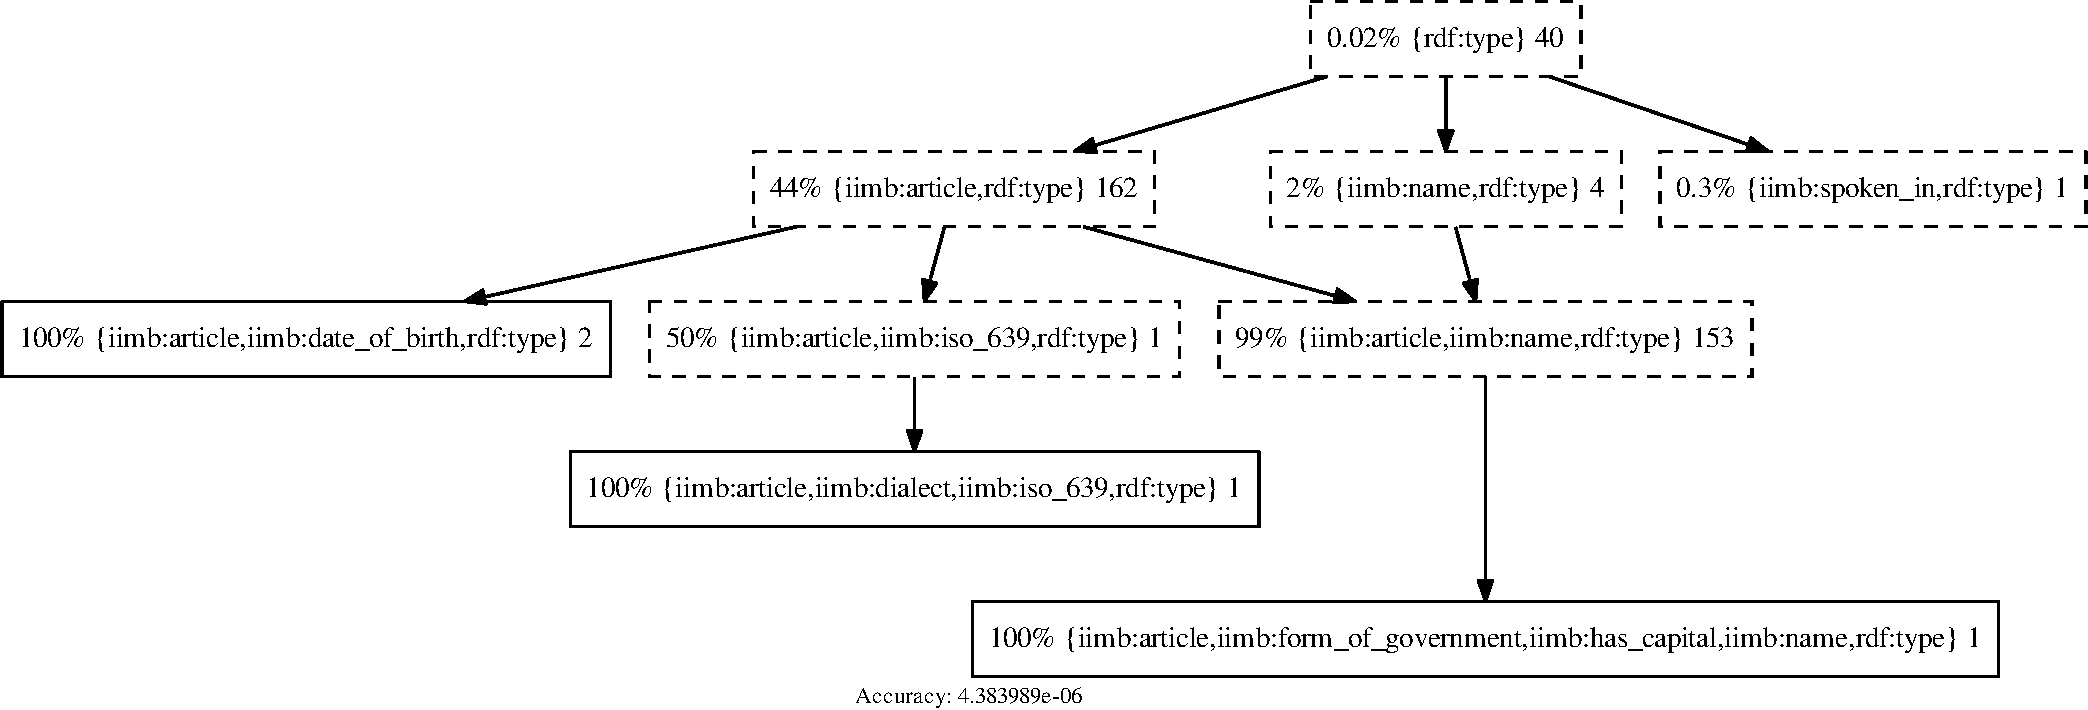
\includegraphics[width=\textwidth]{iimb_approximation_example_crop}
\caption{
  An example of a discernibility partition for an identity relation
    consisting of 365 pairs applied to the fourth IIMB linkset.
  Each node is annotated with the set of predicates $P$ for which
    its pairs are $P$-indiscernible.
  The number of identity pairs within each partition set
    is displayed to the right of the predicate set label.
  Partition sets that contain no identity pair are not show.
  The number that occurs to the left of the predicate label in each node
    indicates how may pairs in that node are identity pairs.
  The lower approximation consists of the nodes with a solid border,
    indicating that they contain only identity pairs.
  The higher approximation consists of all displayed nodes.}
\end{figure*}

\footnote{
  $P$ must be closed under the identity relation, i.e.,
  \begin{equation*}
    cl_{\sim}(P) = \bigcup_{\tuple{\range{p_1}{p_n}} \in P}\nolimits (
      [p_1]_{\sim} \times \ldots \times [p_n]_{\sim}
    )
  \end{equation*}
}
\end{comment}


\subsection{Quality \& Approximation}
\label{sec:approximation}

Not all identity subrelations have the same quality.
Indeed, when we look at the subdivision into three `categories' above,
  we are able to distinguish between a lower approximation of identity,
  as the union of subrelations from the first category
  (definition \ref{def:identity_lower_approximation}),
  and a higher approximation of identity,
  as the union of subrelations from both the first and the second category
  (definition \ref{def:identity_higher_approximation}).

\begin{definition}[Lower approximation]
\label{def:identity_lower_approximation}
\begin{align}
  x \in \lowerapprox
\, \iff \,
    \setdef{y}{x \equiv_{\indp_{\approx}} y}
  \; \subseteq \;
    \approx\nonumber
\end{align}
\end{definition}

\begin{definition}[Higher approximation]
\label{def:identity_higher_approximation}
\begin{align}
  x \in \higherapprox
\, \iff \,
      \setdef{y}{x \equiv_{\indp_{\approx}} y}
    \, \cap \,
      \approx
  \; \neq \;
    \emptyset\nonumber
\end{align}
\end{definition}

\noindent Based on these approximations we can give
  the rough set representation $\pair{\lowerapprox}{\higherapprox}$
  of identity relation $\approx$ \cite{Pawlak1991}.
The quality of a rough set representation is given in
  definition \ref{def:quality}.
The intuition behind this quality measure is that the crispness
  of a set should be proportional to the quality
  of the identity relation on which it is based.
Since a consistently applied identity relation has relatively many
  partition sets that contain either
  no identity pairs (small value for $\lowerapprox$) or
  only identity pairs (large value for $\higherapprox$),
  a more consistent identity relation has a higher accuracy.

\begin{definition}[Quality]
\label{def:quality}
\begin{align}
  \alpha(\approx)
\, = \,
  \dfrac{
    \card{\underline{\sim}}
  }{
    \card{\overline{\sim}}
  }\nonumber
  %\card{\lowerapprox} / \card{\higherapprox}
\end{align}
\end{definition}

\noindent Now that we have a formal metric for quality,
  we can define the characteristics of an ideal identity relation.
Traditionally, the ideal identity relation ensures indiscernibility
  for all expressible properties in the language
  (principle \ref{principle:indiscernibility_of_identicals}).
According to this traditional view, an identity relation becomes of
  higher quality by considering more properties
  according to which two resources are verified to be indiscernible.
We give a different quality criterion by observing that
  for a given identity relation $\approx$,
  defined over a domain of resources $S_G$,
  we can define the notion of full discernibility
  (definition \ref{def:full_discernibility}).

\begin{definition}[Full discernibility]
\label{def:full_discernibility}
A domain $S_G$ is fully discernible with respect to
  a binary relation $\approx$ iff
\[
  \forall x,y \in S_G (
      x \in \equivset{y}
    \lor
      \indp_{\approx}(\equivset{x}) \neq \indp_{\approx}(\equivset{y})
    )
\]
\end{definition}

\noindent From definition \ref{def:full_discernibility}
  it is clear that a domain is fully discernable just in case
  there exists a binary relation $\approx$
  for which \mbox{$\alpha(\approx) = 1.0$}.



\subsection{Example}

\begin{figure*}
\label{fig:ihierarchy}
\centering
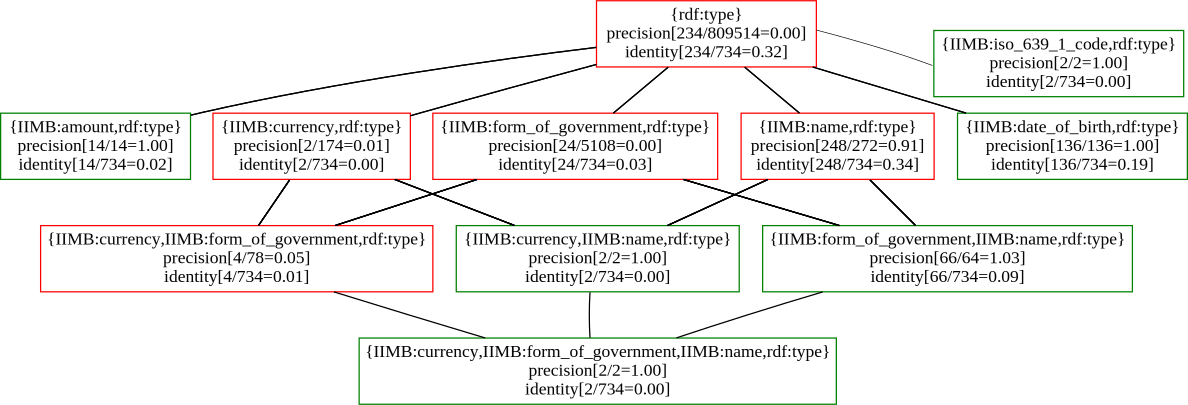
\includegraphics[width=\textwidth]{./img/iimb_16_2}
\caption{
  Example of the identity subrelations for a given dataset (IIMB).
  Each box represents such a subrelation.
  The lower and higher approximation are colored in green and red
    respectively.
  Each box shows the shared predicate terms in curly braces.
  The precision is calculated as
    the number of identity pairs in the subrelation
  divided by
    the number of pairs in the subrelation.
  The identity figure indicates the number of identity pairs in each box,
    divided by the number of identity pairs overall.
}
\end{figure*}

Our approach allows the subrelation hierarchy of a given identity relation
  to be calculated.
Figure \ref{fig:ihierarchy} shows an example of the lower and higher
  approximations for a data- and linkset combination of the IIMB database.
Each rectangular box represents an identity subrelation.
Since in this figure a partition is only drawn when there is at least one
  identity pair that is indiscernible with respect to some set of
  predicates, the higher approximation amounts to the entire figure.
The lower approximation only consists of those partition sets that contain
  at least one identity pair, and that contain no non-identity pair;
  these are distinguished by green borders.


\subsection{Shared properties and indiscernibility}
\label{sec:indiscernibility}

We assume that we are given an identity relation $\approx$,
  which partitions the subject terms $S_G$ according to
  equation \ref{eq:equivalence_set}.

%\small
\begin{equation}
\label{eq:equivalence_set}
  \equivset{x}
=
  \setdef{
    y \in S_G
  }{
    \equivpair{x}{y}
  }
\end{equation}
%\normalsize

%\subsection{Identity relation -> indiscernibility criteria}

Identity can be defined as the smallest equivalence relation,
  i.e. the most fine-grained partition of $S_G$.
For reasoning purposes, mainly the fact that $\approx$
  is an equivalence relation counts.
As we saw in principle \ref{principle:indiscernibility_of_identicals},
  identity implies indiscernibility with respect to all properties.

We can generalize the notion of indiscernibility,
  by parameterizing the set of properties with respect to which
  indiscernibility is determined.
According to this generalization,
  resources $x$ and $y$ are indiscernible with respect to
  a set of properties $P \subseteq P_G \times O_G$
  iff $\forall_{p \in P}(p(x) \leftrightarrow p(y))$ is the case.

It is important to note that every indiscernibility relation
  is also an equivalence relation (reasoning!),
  although not necessarily the smallest one.
Moreover, every indiscernibility relation defined over the domain $S_G$
  is also an identity relation,
  only over a different domain \cite{Quine1950}.\footnote{
    For instance, the set of properties
      ``has an income of $x$ euro's a month''
      for decimals $x$ do not identify people
      (since two people may have the same income),
      but it does identify income groups.
    }

We now reinterpret the identity relation $\approx$,
  as if it were an indiscernibility relation
  whose set of properties $P$ is implicit.
Based on the identity relation,
  we can make the set of properties explicit
  so that $\approx$ becomes an indiscernibility relation.
Definition \ref{def:indiscernibility_properties} makes
  the properties relative to which terms $x_i$ are indiscernibile
  explicit.

\begin{definition}[Indiscernibility properties]
\label{def:indiscernibility_properties}
\begin{align}
  \indpo_{\approx}(\set{\range{x_1}{x_n}})
=
  \setdef{
    \pair{p}{o} \in P_G \times O_G
  }{\nonumber\\
    \bigwedge_{1 \leq i \leq n}
      \exists p_i \in \equivset{p},
        \exists o_i \in \equivset{o}(
          \triple{x_i}{p_i}{o_i} \in G
        )
% Alternatively, we can place the quantifies outside the conjunction:
%    \exists_{\range{p_1}{p_n} \in \equivset{p}},
%      \exists_{\range{o_1}{o_n} \in \equivset{o}}
%        \bigwedge_{1 \leq i \leq n} \triple{x_i}{p_i}{o_i} \in G
  }\nonumber
\end{align}
\end{definition}

\noindent Notice that in definition \ref{def:indiscernibility_properties}
  we close both the predicate terms $p$ and the object terms $o$
  under identity.
This may be important,
  since ``Berlin'' and ``Berlijn'' (i.e., the Dutch spelling of ``Berlin'')
  may denote identical resources, as may ``lives in'' and ``woont in''
  (i.e., the Dutch spelling of ``lives in'').
When being given data stating that ``Person $a$ lives in Berlin''
  ``Person $b$ woont in Berlijn'', $a = b$, $\text{Berlin} = \text{Berlijn}$,
  and $\text{lives is} = \text{woont in}$,
  we want to identify the permutations of
  $\set{\text{lives in},\text{woont in}}$ and
  $\set{\text{Berlin},\text{Berlijn}}$
  as the indiscernibility properties.

Using definition \ref{def:indiscernibility_properties},
  we can deduce that the indiscernibility properties for
  the identity pair $\pair{\text{Amsterdam}}{\text{Berlin}}$
  would contain (amongst many others) the properties
  ``is a city'', ``has more than 100,000 inhabitants'', and
  ``is located in Europe''.

But we are not only interested in the properties that resources share
  with one other (e.g., being a city, having more than 500,000 inhabitants).
We are also interested in the predicates that a set of resources share.
This amounts to a simple abstraction of
  definition \ref{def:indiscernibility_properties},
  equating the sets of objects (closed under identity)
  and only returning the set of shared RDF predicate terms
  (see definition \ref{def:indiscernibility_predicates}).

\begin{definition}[Indiscernibility predicates]
\label{def:indiscernibility_predicates}
\begin{align}
  \indp_{\approx}(\setrange{x_1}{x_n})
=
  \setdef{
    p \in P_G
  }{
    \exists_{\range{p_1}{p_n} \in \equivset{p}}(\\
        \equivset{
          \setdef{
            o \in O_G
          }{
            \triple{x_1}{p_1}{o}
          }
        }
      =
        \ldots
      =
        \equivset{
          \setdef{
            o \in O_G
          }{
            \triple{x_n}{p_n}{o}
          }
        }
    )
  }\nonumber
\end{align}
\end{definition}

We are also interested in resource pairs that share their sharing properties.
We can thus identify subsets of an identity relation based on differences
  in the sets of predicate path maps relative to which they take resources
  to be \emph{indiscernible} from one another.


We call the predicates that are shared by a set of identical resources $X$
  the indiscenibility criteria for $X$
  (def. \ref{def:indiscernibility_criteria}).

EXAMPLE HERE (PREFERABLY IIMB).

\begin{comment}
Drawing:
<s,p,o1>
<s,p,o2>
<o1,=,o2>
From IIMB data.
\end{comment}

\subsection{Indiscernibility criteria -> identity subrelation}

When we look at the triples that constitute a set of identity relations,
  we see that all identity assertions look the same.
But when we take the properties of those identical resources into account,
  we observe that within a given identity relation there can be different
  subrelations that can be characterized by different sets of properties.

For instance, in the IIMB dataset there are some identical resources that
  share the property \verb|IIMBTBOX:spoken_in|, while other pairs share
  the property \verb|IIMBTBOX:form_of_government|.
The set of pairs of resources that are spoken in the same language may even
  be disjoint from the set of pairs of resources that have the same
  form of government, indicating identity according to different criteria.
In this example, one subset of the identity relation does not discern
  resources that are spoken in the same language, whereas another subset
  of the identity relation does not discern resources that have the same
  form of government.

We say that two resource pairs are indiscernible
  in case both pairs are indiscernible for the same
  $P \subseteq \powerset{P_G}$
  (def. \ref{pair indiscernibility}).

\subsection{Indiscernibility partition -> identity subrelations}

Based on the indiscernibility criteria,
  i.e. the sets of properties that are shared by identical resources,
  we can derive those resource pairs that share
  the same sharing properties.
We can thus identify subsets of an identity relation based on
  differences in the sets of properties relative to which
  the resource pairs that they consist of are
  (in)discernible from one another.
Identity of indiscernibility criteria provides
  another equivalence relation
  ($\approx_{\indp}$, def. \ref{def:indiscernibility_partition}),
  that partitions the identity relation $\approx$ into
  identity subrelations that characterize identity based on different
  indiscernibility criteria.

\begin{definition}[Indiscernibility partition]
\label{def:indiscernibility_partition}
\begin{align}
  \approx_{\indp}
=
  \setdef{
    \pair{\pair{x_1}{x_2}}{\pair{y_1}{y_2}} \in (S_G^2)^2
  }{\\
    \indp_{\approx}(\set{x_1,x_2}) = \indp_{\approx}(\set{y_1,y_2})
  }\nonumber
\end{align}
\end{definition}


\footnote{
  $P$ must be closed under the identity relation, i.e.,
  \begin{equation*}
    cl_{\sim}(P) = \bigcup_{\tuple{\range{p_1}{p_n}} \in P}\nolimits (
      [p_1]_{\sim} \times \ldots \times [p_n]_{\sim}
    )
  \end{equation*}
}

\small
\begin{definition}[Indiscernibility]
\begin{align}
\label{def:resource_indiscernability}
\mathit{IND}(P) \,=\,
  \setdef{
    \pair{x}{y} \in S_G^2
  }{
    \forall_{p \in cl_{\sim}(P)} f_p(x) \approx f_p(y)
  }
\\
\label{pair indiscernibility}
\mathit{IND}(P^*) \,=\,
  \setdef{
    \pair{\pair{x_1}{y_1}}{\pair{x_2}{y_2}} \in (S_G^2)^2
  }{\\
    \forall_{P \in P^*}
        \pair{x_1}{y_1} \in \mathit{IND}(P)
      \leftrightarrow 
        \pair{x_2}{y_2} \in \mathit{IND}(P)
  }\nonumber
\end{align}
\end{definition}
\normalsize

\noindent According to the standard definition,
  identical resources are indiscernible with respect to all properties.
We take a given set of identity pairs and partition it into subsets which
  we can describe as being $cl_{\sim}(P)$-indiscernible,
  for $P \subseteq P_G^n$.

Fig. 1 shows an example
  of a discernibility partitioning for a given identity relation.

\begin{comment}
\begin{figure*}
\label{fig:iimb_example}
\centering
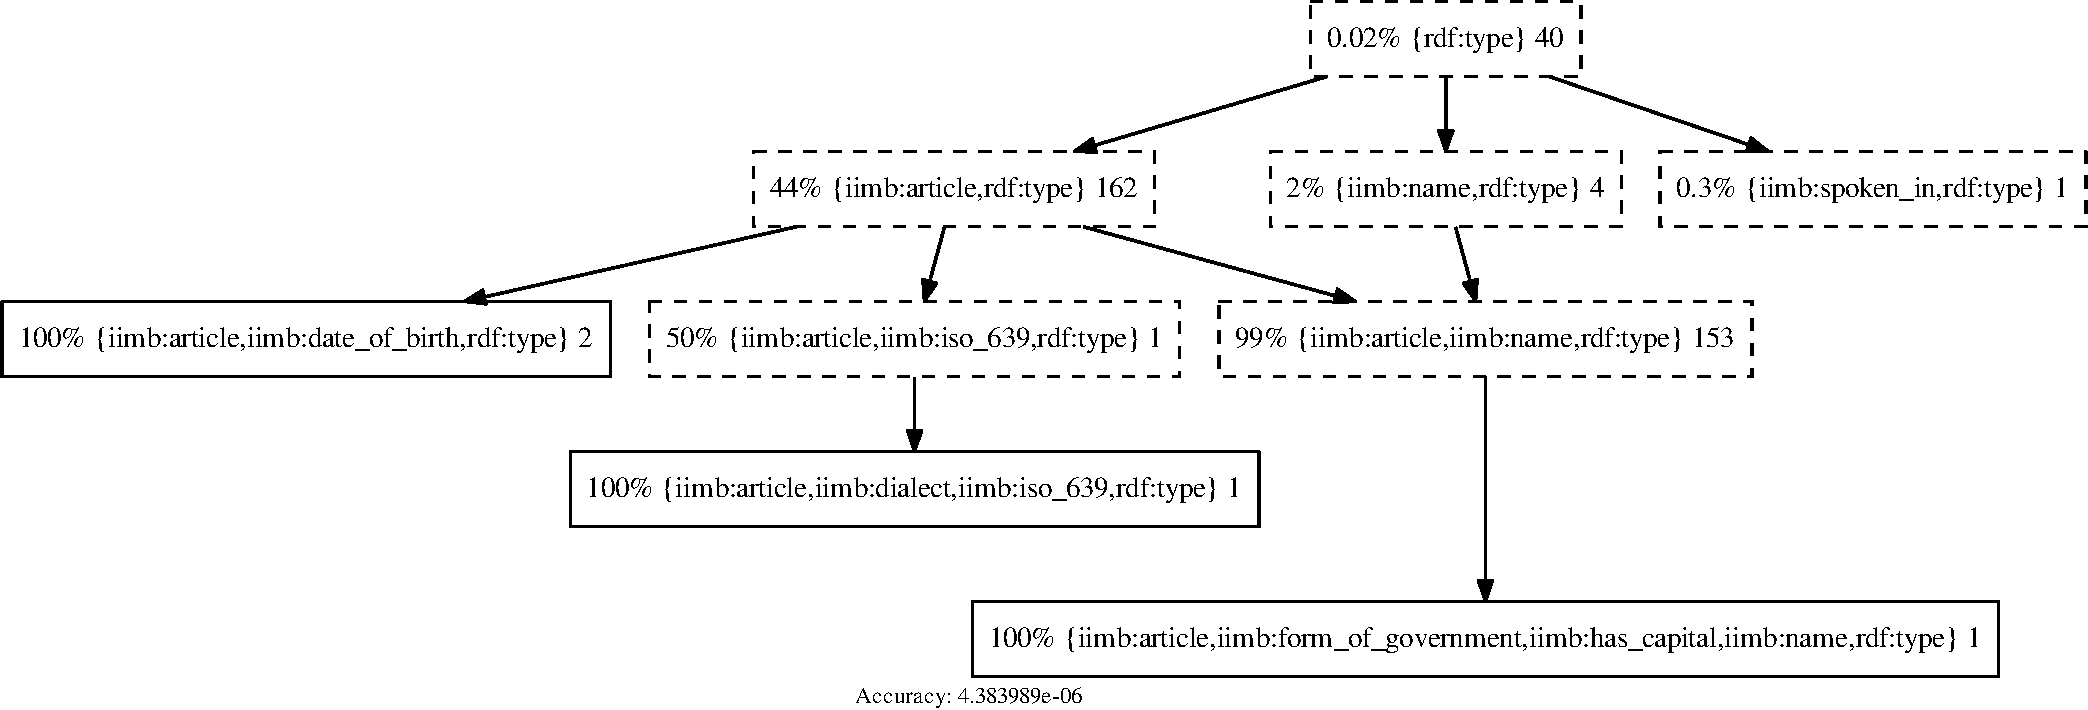
\includegraphics[width=\textwidth]{iimb_approximation_example_crop}
\caption{
  An example of a discernibility partition for an identity relation
    consisting of 365 pairs applied to the fourth IIMB linkset.
  Each node is annotated with the set of predicates $P$ for which
    its pairs are $P$-indiscernible.
  The number of identity pairs within each partition set
    is displayed to the right of the predicate set label.
  Partition sets that contain no identity pair are not show.
  The number that occurs to the left of the predicate label in each node
    indicates how may pairs in that node are identity pairs.
  The lower approximation consists of the nodes with a solid border,
    indicating that they contain only identity pairs.
  The higher approximation consists of all displayed nodes.}
\end{figure*}

\footnote{
  $P$ must be closed under the identity relation, i.e.,
  \begin{equation*}
    cl_{\sim}(P) = \bigcup_{\tuple{\range{p_1}{p_n}} \in P}\nolimits (
      [p_1]_{\sim} \times \ldots \times [p_n]_{\sim}
    )
  \end{equation*}
}
\end{comment}


\subsection{Quality \& Approximation}
\label{sec:approximation}

Not all identity subrelations have the same quality.
Indeed, when we look at the subdivision into three `categories' above,
  we are able to distinguish between a lower approximation of identity,
  as the union of subrelations from the first category
  (definition \ref{def:identity_lower_approximation}),
  and a higher approximation of identity,
  as the union of subrelations from both the first and the second category
  (definition \ref{def:identity_higher_approximation}).

\begin{definition}[Lower approximation]
\label{def:identity_lower_approximation}
\begin{align}
  x \in \lowerapprox
\, \iff \,
    \setdef{y}{x \equiv_{\indp_{\approx}} y}
  \; \subseteq \;
    \approx\nonumber
\end{align}
\end{definition}

\begin{definition}[Higher approximation]
\label{def:identity_higher_approximation}
\begin{align}
  x \in \higherapprox
\, \iff \,
      \setdef{y}{x \equiv_{\indp_{\approx}} y}
    \, \cap \,
      \approx
  \; \neq \;
    \emptyset\nonumber
\end{align}
\end{definition}

\noindent Based on these approximations we can give
  the rough set representation $\pair{\lowerapprox}{\higherapprox}$
  of identity relation $\approx$ \cite{Pawlak1991}.
The quality of a rough set representation is given in
  definition \ref{def:quality}.
The intuition behind this quality measure is that the crispness
  of a set should be proportional to the quality
  of the identity relation on which it is based.
Since a consistently applied identity relation has relatively many
  partition sets that contain either
  no identity pairs (small value for $\lowerapprox$) or
  only identity pairs (large value for $\higherapprox$),
  a more consistent identity relation has a higher accuracy.

\begin{definition}[Quality]
\label{def:quality}
\begin{align}
  \alpha(\approx)
\, = \,
  \dfrac{
    \card{\underline{\sim}}
  }{
    \card{\overline{\sim}}
  }\nonumber
  %\card{\lowerapprox} / \card{\higherapprox}
\end{align}
\end{definition}

\noindent Now that we have a formal metric for quality,
  we can define the characteristics of an ideal identity relation.
Traditionally, the ideal identity relation ensures indiscernibility
  for all expressible properties in the language
  (principle \ref{principle:indiscernibility_of_identicals}).
According to this traditional view, an identity relation becomes of
  higher quality by considering more properties
  according to which two resources are verified to be indiscernible.
We give a different quality criterion by observing that
  for a given identity relation $\approx$,
  defined over a domain of resources $S_G$,
  we can define the notion of full discernibility
  (definition \ref{def:full_discernibility}).

\begin{definition}[Full discernibility]
\label{def:full_discernibility}
A domain $S_G$ is fully discernible with respect to
  a binary relation $\approx$ iff
\[
  \forall x,y \in S_G (
      x \in \equivset{y}
    \lor
      \indp_{\approx}(\equivset{x}) \neq \indp_{\approx}(\equivset{y})
    )
\]
\end{definition}

\noindent From definition \ref{def:full_discernibility}
  it is clear that a domain is fully discernable just in case
  there exists a binary relation $\approx$
  for which \mbox{$\alpha(\approx) = 1.0$}.



% Section 3: Experiments
\section{Experimental Validation}
\label{sec:experiment}
\label{sec:experimental_design}
\label{sec:experimental_validation}

In order to subject our theory to an experimental test,
  we use the IIMB dataset\footnote{\URL{islab.di.unimi.it/iimb}}
  that is used in the
  instance matching track of the 2012 Ontology Alignment Evaluation
  Initiative (OAEI\footnote{\URL{oaei.ontologymatching.org}}).
This dataset consists of eighty ontologies $G_i$ (for $1 \leq i \leq 80$)
  that are linked to a single base ontology $G_0$.
The identity links between $G_0$ and $G_i$ are annotated with a
  confidence measure between $0.0$ and $1.0$.
A graph $G$ is the result of fully materializing the graph merge
  of $G_i$ (for some $1 \leq i \leq 80$) and $G_0$.
For each of these eighty linked ontologies a reference mapping is available.

In our experiment we ran separate tests for each of the $80$ datasets
  and took the average values for incremental reductions of
  random parts of the identity relations between $G_0$ and the $80$
  different $G_i$'s.
In other words we deliberate make the identity relation incomplete.
We then calculate the rough set representation using this altered relation.
We then evaluate how many of the removed identity pairs occur in
  the higher approximation.
Our hypothesis is that the percentage of removed identity pairs
  in the higher approximation is larger than the percentage of pairs
  in the higher approximation.
If the hypothesis is validated, this indicates that
  calculating the rough set representation for a partial identity relation
  would indeed improve suggestions for extending that identity relation.

Since the data may contain noise, using precision degrees $0.0$ and $1.0$
  may be too strict. For this experiment we have set these boundaries
  to $0.05$ and $0.95$ respectively.

Figure \ref{fig:recall_quality} shows the different behaviours of the
  upper and lower approximations, with the upper approximation indeed
  having a dramatically higher recall than the lower approximation.

\begin{figure}
\centering
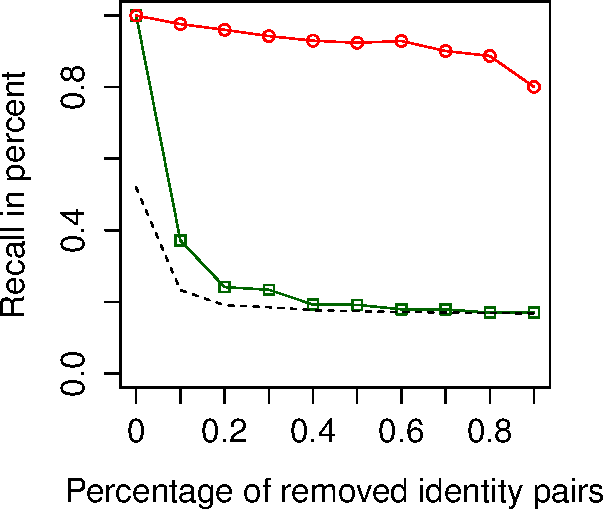
\includegraphics[width=0.8\linewidth]{./img/recall_quality}
\caption{
  The recall of the lower and higher approximation
    are shown by the green line (circles) and red line (boxes) respectively.
  The quality metric (definition \ref{def:quality})
    is shown by the dashed line.
}
\label{fig:recall_quality}
\end{figure}

In figure \ref{fig:in_higher}
  we see that the randomly removed identity pairs are often
  in the higher approximation, even when large parts of
  the identity relation are removed.

\begin{figure}
\centering
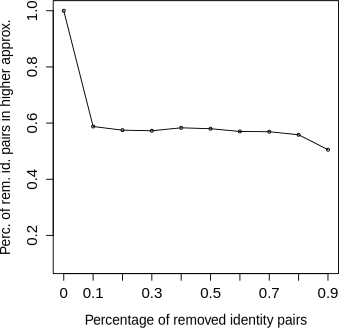
\includegraphics[width=0.8\linewidth]{./img/in_higher}
\caption{
  The percentage of the removed identity pairs that are in the higher approximation
}
\label{fig:in_higher}
\end{figure}

\begin{comment}
Lower recall
1.0,0.37172100183246687,0.24123550044617229,0.23375413992878838,0.19251810221158194,0.1916729296953922,0.1790536768898471,0.17912482945205316,0.1696252362320524,0.17011849853438268
Higher recall
1.0,0.976185052819561,0.9600384749021372,0.9425765362723856,0.9297564861502547,0.9239282325982691,0.9288077551757412,0.900878631549093,0.886987450993775,0.8005503359226204
Quality
0.5190405227795084,0.23261438049447705,0.1904353344556299,0.18505145463363135,0.17658153004935476,0.17387635867899948,0.17168948193128328,0.17017370794837366,0.16844506704419984,0.1677780567227606
Higher cover
0.0006413304103753317,0.0006098495555258293,0.0005825544051162525,0.0005747252831024628,0.0005640718998200667,0.0005626590987592347,0.0005613753926606205,0.0005464403973849621,0.0005372610299329459,0.00046916805031848495
Removed identity pairs in higher
1.0,0.5877680311890837,0.5747530425162004,0.572660333493667,0.5831761670185315,0.5799385908868745,0.5701984042084377,0.5692284399224807,0.558405393333526,0.5051324217787632
\end{comment}



\subsection{Future Experiments}
\label{sec:hypotheses}

Space limitations do not allow us to describe the results of further
  experiments. Instead, we will describe some of the other hypotheses
  that can be evaluated using our approach:
\begin{enumerate}
\item Take an {\small \texttt{owl:sameAs}} relation and
        a {\small \texttt{skos:related}}
        relation defined over the same domain.
      Merge them into a new binary relation $\sim$.
      Establishing the lower and higher approximation of $\sim$,
        the hypothesis is that pairs from {\small \texttt{owl:sameAs}}
        occur more frequently in the lower boundary than pairs from
        {\small \texttt{skos:related}},
\item Take a set of alignment pairs, each of which is associated with
        a confidence measure between $0.0$ and $1.0$.
      Choose an arbitrary cutoff point $0.0 < c < 1.0$.
      The hypothesis is that alignments with a confidence larger than $c$
        occur more frequently in the lower approximation than alignments
        with a confidence smaller than $c$.
\item Take a set of automatically generated alignment pairs with
        associated confidence measures and take the gold standard or
        reference alignment for the same dataset.
      The hypothesis is that pairs that occur in the lower approximation
        of the alignment appear relatively more often in the gold standard
        than pairs that occur in the higher approximation of the alignment.
\item The quality measure $\alpha$ of a reference alignment is generally
        higher than the accuracy measure of an automatically generated
        alignment for the same dataset.
      Or, the quality measure is generally higher for identity relations
        that domain experts consider to be correct.
\end{enumerate}

\noindent Finally, the IIMB datasets are quite small
  (tens of thousands of triples).
We will have the verify whether the current implementation is able to scale
  to bigger datasets.


% Section 4: Conclusion
\section{Conclusion}
\label{sec:conclusion}

In this paper we have given an new approach for characterizing,
  extending/retracting, and assessing identity relations.
Our approach does this in purely qualitative terms, using schema semantics.
In contemporary ontology alignment and data linking activities nonsemantic
  aspects of resources play a role as well.
For instance similarity assessment for natural language labels is often
  used in data linking.

We think that the qualitative means of characterizing an identity relation
  are a useful addition to existing quantitative means.
Also, we think that it is more useful and viable to enrich existing
  identity relations in the LOD based on the semantics of the datasets
  in which they occur, than to introduce new relationships into SW languages.
Apart from the practical difficulties of teaching practitioners
  and transforming/enriching existing datasets, we suggest that the
  meaning of an identity (sub)relation is partially defined in its use,
  i.e., in the indiscernibility criteria it embodies.

For our approach it is not necessary to pose additional restrictions
  on a binary relation $\sim$.
The definitions in this paper apply to \verb|owl:sameAs| relations
  in the same way in which they apply to any other binary relation
  (e.g., \verb|skos:related|).

We are currently in the process of validating the above enumerated hypotheses.
The results of these evaluations are continuously being published on
  \verb|wouterbeek.com/identity-on-the-web|.
The website currently contains the automated results of all eighty IIMB
  alignments, drawn from the instance matching track of the
  OAEI 2012.
The website also refers to the publicly available Git repository
  \verb|github.com/wouterbeek/IOTW| where the implementation
  discussed in section \ref{sec:implementation} can be found.

%\input{./tex/futurework.tex}

% Bibliography
\bibliographystyle{aaai}
\bibliography{kr2014_iotw}

\end{document}
